% Created 2022-07-29 Fri 23:25
% Intended LaTeX compiler: pdflatex
\documentclass{article}
\author{arcotpixel}
\date{\today}
\title{}
\begin{document}

\section*{Syndrome Sinistre: Left Brachiocephalic Vein Compression and its Neurolgical Manifestations.}
\label{sec:org47e8791}
\section*{Background:}
\label{sec:orge916ee1}
Embryologically, the left brachiocephalic vein (LBV) originates as an anastamotic channel between the right and left \emph{anterior} cardinal veins (Mozes, GEZA and Gloviczki, PETER, 2007).
This positions the LBV between the manubrium sterni anteriorly and the innominate artery posteriorly (Standring, Susan, 2015).
This pattern of adjacency of the aorta to the LBV is unique to mammals and results from a quirk of evolution (Hirokawa, Nobutaka and Tanaka, Yosuke and Okada, Yasushi, 2009).
With age, the ascending aorta, unfolds, elongates and dilates (Ohyama, Yoshiaki and Redheuil, Alban and Kachenoura, Nadjia and Ambale Venkatesh, Bharath and Lima, Joao A.C., 2018).
Simultaneously, there is a change in the thoracic geometry that reduces the thoracic volume primarily from disc height loss and kyphosis (Holcombe, Sven A. and Wang, Stewart C. and Grotberg, James B., 2017).
These transitions progressively compress the LBV. Normally this compression is circumvented via collateral pathways and "Blood finds a way" (Marini, Thomas J. and Chughtai, Komal and Nuffer, Zachary and Hobbs, Susan K. and Kaproth-Joslin, Katherine, 2019).
However "What if these collaterals are insuffcicient?" is a question that has not been answered. It is possible that there is no clinical detriment and this is just an innocuous finding.
On the contrary, it may signal a whole class of neurological disorders and explain the pathophysiology of hitherto unexplained neurological and neurodegenrative conditions.

\section*{Embryology, Anatomy and Radiology:}
\label{sec:orgc96e9bd}
The anterior cardinal veins drain the cephalic portion of the embryo.
During week eight of development the thyroid and thymic veins join to form a large transverse anastamosis superior to the common cardinal veins.
This anastamosis allows blood from the cephalic portion of left anterior cardinal vein (future left internal jugular vein) to reach the junction of the right anterior cardinal vein (future right internal jugular vein) and right common cardinal vein (future superior venacava (SVC)).
Various developmental venous malformations (left sided SVC, double SVC) may occur if the above does not proceed according to plan (White, Hunter J. and Soos, Michael P., 2022).
Normally however, one ends up with an efficent LBV that transports blood from the left internal jugular vein to the superior vena cava.
Until, of course, it is smothered by its more sturdy neighbours.

The LBV vein is approximately 6 cm to 7 cm long.
It is formed by the confluence of the left internal jugular vein and the left subclavian vein behind the left sternoclavicular joint.
It then runs and obliuqe and downward course to the right to join the right brachiocephalic vein and form the superior vena cava behind the sternum and the first intercostal space.
In its course, it receives the the following veins: left  vertebral, left inferior thyroid, left internal thoracic, left superior intercostal, left supreme intercostal, thymic and pericardiacophrenic veins.
Its relations with its less compliant neighbours forms the crux of this syndrome.
It initially runs anterior to the parietal pleura of the lung and then enters a valley between the bony manubrium anteriorly and an unyielding innominate artery posteriorly (Standring, Susan, 2015).
It is in this valley that the LBV gets trapped usually for a few millimeters congruent with the portion in contact with the innominate artery.

The radiological findings are often obvious but the apparent lack of clinical relevance lends to under reporting.
As an example, osteporotic vertebral fractures suffer a similar fate (Williams, Alexandra L. and Al-Busaidi, Aisha and Sparrow, Patrick J. and Adams, Judith E. and Whitehouse, Richard W., 2009).
There are excellent examples of LBV compression with resultant venous reflux on CT angiography (Seth, Raghav and Bhatia, Vikas and Jain, Chirag and Kumar, Ajay, 2022,  Tseng, Ying-Chi and Hsu, Hui-Ling and Lee, Tsong-Hai and Chen, Chi-Jen, 2007).
Similar findings are noted on MR Venography (Han, Ke and Chao, A.-Ching and Chang, Feng-Chi and Chung, Chih-Ping and Hsu, Hung-Yi and Sheng, Wen-Yung and Wu, Jiang and Hu, Han-Hwa, 2015).
Conventional catheter based venography is a poor modality to detect this condition, as the plane of compression is usually parallel to the antero-posterior plane and the lateral plane is obscured by the patients arms.
Intravascular ultrasound however should be the new "gold standard" as it clearly identifies and demonstrates the dramatic decrease in luminal area while providing accurate vesel measurements that are necessary for treatment.
This condition will continue to elude detection by CT angiography, if right sided injections are performed (Tseng, Ying-Chi and Hsu, Hui-Ling and Lee, Tsong-Hai and Chen, Chi-Jen, 2007) and MR venography of the neck if coverage does not extend down to the level of the LBV.

\begin{center}
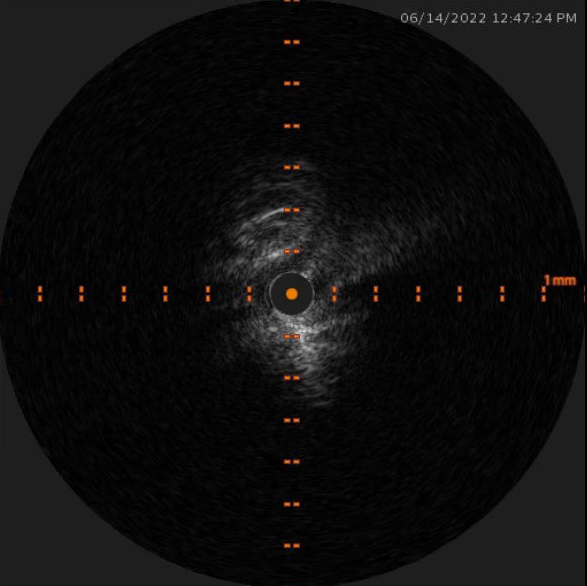
\includegraphics[width=.9\linewidth]{./images/LBV-Compression.png}
\end{center}



\section*{Discussion:}
\label{sec:orgd0b82ee}
LBV compression should be expected to occur and progress with aging due to the anatomical factors described above.
It should generally be asymptomatic given the remarkable redundancy of the venous system and its collaterals.
Symptoms should and do ensue when the venous collaterals are either insufficient or overwhelmed.
This can be compounded by venous obstruction on the contralteral side, which is not uncommon.
For example, trapping of the right internal jugular vein at the level of the C1 transverse process which is commonly noted in a similar age group.
In fact it might be necesary for bilateral outflow obstruction given the robust nature of the connections between the dural sinuses.
This results in the emergence of two pathophysiological states.
One governed by a build up of pressure due to venous hypertension and the other governed by stagnation / venous congestion.
The venous hypertensive state could potentially explain the mechanical effects such as headache and disorders that arise from obstruction of csf.
Accumulation of toxic waste metabolites (Cheng, Yiming and Haorah, James, 2019) due to poor venous outflow could potentially explain the chemical effects that lead to neurological dysfunction or even neurodegenration.
Clinically, in my experience, there appears to be a predeliction for headaches, vertigo, tinnitus, deafness and imbalance.
Ageing is a risk factor for neurodegenerative disease (Hou, Yujun and Dan, Xiuli and Babbar, Mansi and Wei, Yong and Hasselbalch, Steen G. and Croteau, Deborah L. and Bohr, Vilhelm A., 2019) and ageing is a risk factor for LBV compression.
Is it possible that the LBV compression is an important precursor of neurodegenrative diseases?

\section*{Conclusion:}
\label{sec:org4c1a14a}
There have been multiple attempts to link singular neurological disorders to venous outflow obstruction.
The obverse, multiple neurological manifestations from a single site of obstruction,  might be the closer to reaslity.
The prime example was chronic cerebro spinal venous insufficiency which tied itself to multiple sclerosis (Zamboni, P and Galeotti, R and Menegatti, E and Malagoni, A M and Tacconi, G and Dall’Ara, S and Bartolomei, I and Salvi, F, 2009).
It was heralded by a flurry of research which simply imploded when the initial results were not widely repoducible (Baracchini, Claudio and Valdueza, José M. and Del Sette, Massimo and Baltgaile, Galina and Bartels, Eva and Bornstein, Natan M. and Klingelhoefer, Juergen and Molina, Carlos and Niederkorn, Kurt and Siebler, Mario and Sturzenegger, Matthias and Ringelstein, Bernd E. and Russell, David and Csiba, Laszlo, 2012).
This may have been responsible for the general perecption of dubiousness and outright opposition to venous procedures for neurological disorders.
As another example, transverse sinus stenosis as a cause of intracranial hypertension, is a more recent association that appears in need of definitive evidence to become widely accepted (Gurney, Sam P. and Ramalingam, Sateesh and Thomas, Alan and Sinclair, Alex J. and Mollan, Susan P., 2020).
The list continues on with conditions such as transient global amnesia (Han, Ke and Chao, A.-Ching and Chang, Feng-Chi and Chung, Chih-Ping and Hsu, Hung-Yi and Sheng, Wen-Yung and Wu, Jiang and Hu, Han-Hwa, 2015), deafness (Griffith, Adrian N, 1961), Normal Pressure Hydeocephalus (Satow, Takeshi and Aso, Toshihiko and Nishida, Sei and Komuro, Taro and Ueno, Tsukasa and Oishi, Naoya and Nakagami, Yukako and Odagiri, Masashi and Kikuchi, Takayuki and Yoshida, Kazumichi and Ueda, Keita and Kunieda, Takeharu and Murai, Toshiya and Miyamoto, Susumu and Fukuyama, Hidenao, 2017) and so on.

One could argue that a more holistic approach is in order.
If such an approach was applied, the entire class of disorders, neurological or otherwise would come under an umbrella term such as Venous Outflow Obstruction Disorders (Voodoo).
The venous hierarchy (for the superior vena caval system) would be along anatomical lines beginning with the cortical veins, coursing through the superior sagittal, inferior sagittal and straight sinuses, moving on to the transverse and signoid sinuses, followed by the paired jugular and brachiocephalic veins with the superior venacava and the right heart, pulmonary arteries and left heart forming the inferior portions.
Theoretically, any dowstream segment in the hierarchy should be able to affect any upstream segment and produce a congruent disorder.
For example, one should not be surprised when superior vena caval stenosis produces papilledema in a patient and similarly not be surprised if transverse sinus stenting does not relieve the papilledema in said patient.
Thus it would be important to evaluate the entire pathway and treat tandem lesions, in some cases bilaterally in order to restore good venous outflow from both the superficial and deep pathways.

LBV compression would fall into this class of disorders. The neurological symptoms would depend on the drainage pathway that was affected.
On the surface, this condition  appears to associated with seemingly innocuous complaints such as headache and vertigo.
At a deeper level it may be a precursor of more sinister neurodegenerative disorders.
Given the technical ease of its treatment with stenting, it represents a serious target for further research along with other venous outflow obstruction disorders.
\end{document}